\chapter{Perceptual Quality}\label{chap:02}

\section{Perception and Psychophysics}
Human use their senses, \ie, perceptual organs, to perceive events of their environment.
Based upon perceived events an internal model is created and updated, which incorporates knowledge about the environment and thus reality.
This model is then used to plan actions and updated when new information including perceptual events are processed~\citep[p. 4]{blauert_spatial_1996}.
A \emph{perceptual event} occurs in a human observer, when a \emph{physical event} stimulates a sensory organ~\citep{blauert_spatial_1996}.
A physical event is an observable occurrence in time, location and character~\citep{callet_qualinet_2013}.
%One example of a physical event is a sound event that reaches the ear results in an auditory event in the observer (see \autoref{img:chap02:auditory-event}).
As the perceptual event occurs inside the observer due to perceptual and mental processing, it cannot observed directly.
A perceptual event can be described by the observer by comparing the perception to other known features and express it.
By measuring the properties of a physical event and relating those measurements to the description of the perceptual events psychometric functions can be derived.
In fact, the perception of a physical event may change the internal state of an observer.
The physical event reaching the sensory organ can affect the sensitivity or the observer might react to a physical event and thus affect the perception of following physical events.
The perception of different physical events is not only affected by the temporal order, but temporal close physical events may grouped together and form one perceptual event.

A psychophysical experiment is conducted by presenting one or more physical events as stimuli to one or more observers.
Each individual observer derives the description of his perceptual event.
The description can be expressed in a quantitative form by selecting the best fitting answer from a pre-defined set or in a free form.
Whereas in the first case the encoding is conducted by an observer himself, in the latter case the encoding open by the observer.
In addition to variations in the perception process leading to varying perception also the observation and description process may change.
The description of a physical event and their perception must not necessarily be identical for different observers as each observer describes his individual perceptual event~\citep[p. 11]{blauert_spatial_1996}.
A psychophysical experiment is considered \emph{objective}, if the results are reproducible, independent if one participant is measured repeatedly or multiple participants are used~\citep[p. 11]{blauert_spatial_1996}.
However, the description task requires that the perceptual event can be observed consciously and an \emph{active} observation process may affect the actual perception and thus perceptual event.
In the description process the order of stimuli might affect the description as previous stimuli can be used as reference), but it might changes over longer time spans as more information could be memorized.

\section{Perceptual Quality and Quality Formation Process}
The field \emph{perceptual quality}, or so-called \ac{QoE}, is a field of psychophysics focusing on the \emph{experience} due to perception and the resulting \emph{quality} of this experience.
\begin{definition}[Experiencing]
``is the individual stream of perceptions (of feelings, sensory percepts and concepts) that occurs in a particular situation of reference.''~\citep[p. 13]{moller_quality_2014}.
\end{definition}

With regard to quality of an experience, and the underlying perceptual events, \cite{jekosch_voice_2005} formulates the \emph{quality formation process} as individual comparison process between the desired outcome, or expected, with the experienced outcome.
The comparison with the expectations of the experience results in a \emph{quality event} in the observer.
This complements the description of a perceptual event by an additional quality evaluation process.
This process is shown in \autoref{img:chap02:quality-event}.
\begin{figure}
	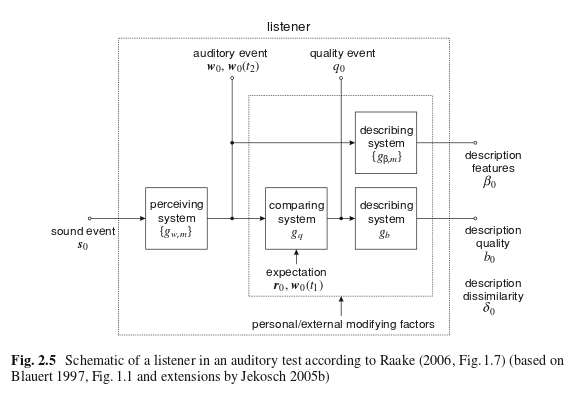
\includegraphics[width=1\textwidth]{figure/quality-event}
	\caption{Quality formation and description process as extension to the perceptual event.}
	\label{img:chap02:quality-event}
\end{figure}

It is assumed that a perceptual event is evaluated by the comparing system within an observer with regard to the \emph{quality features} of this event~\citet[\cf p. 17]{jekosch_voice_2005}.
\footnote{\citet{jekosch_voice_2005} uses the term \emph{entity} with regard to the quality formation process.
As entity does not convey a temporal component, the term \emph{event} is in this work used instead following the notion of \cite{blauert_spatial_1996} although the duration of an event is not considered there.}

\begin{definition}[Quality Feature]
``A quality feature is a recognized and designated characteristic of an entity that is relevant to the entity's quality.''~\citep[p. 17]{jekosch_voice_2005}
\end{definition}

It is assumed that the evaluation of the difference between the \emph{perceived quality features} and the \emph{desired quality features} result in a the experienced quality~\citet[p. 23]{raake_book}.
With regard to telecommunication services and multimedia systems the term \emph{perceived quality} has been extended to \acf{QoE}.
In \ac{QoE} an observer is not only regarded as a measurement instrument, but as an actor striving for a \emph{satisfying} perceived quality with regard to his expectations, requirements and needs.
In difference to an observer, who only describes an event, in \ac{QoE} the perceiving human is regarded as an actor that can not only react but also proactive make decisions.

\begin{definition}[\acf{QoE}]
``is the degree of delight or annoyance of a person whose experiencing involves an application, service, or system.
It results from the person’s evaluation of the fulfillment of his or her expectations and needs with respect to the utility and / or enjoyment in the light of the person’s context, personality and current state.''~\citep[p. 21]{moller_quality_2014}.
\end{definition}

\citet{raake_speech_2006} and \citet{moller_quality_2014} extended the \emph{quality formation process} of \citet{jekosch_voice_2005}.
Raake splits the quality formation process into three phases as shown in \autoref{img:chap02:quality-formation-process}.
The first phase contains the sensory processing depending on contextual information and predescessing perceptual events, which transforms a physical event to a perceptual event leading to the perceived characteristic.
This phase also contains reactions to the perceptual event by exploration and anticipation.


\begin{definition}[Assumed Quality]\label{def:assumedquality}
``corresponds to the quality and quality features that users, developers, manufacturers or service providers assume regarding a system, service or product that they intend to be using, or will be producing, without however grounding these assumptions on an explicit assessment of \textit{quality based on experiencing}.''~\citep[p. 20]{moller_quality_2014}.
\end{definition}

%Geerts - Meta-Framework merging:
%% User, Product, Use Process(Wright: identification, incorperation, identification; non-use/abondonment!), Context (\cf Mantovani)
%% WRIGHT. Micro (in one session): anticipating, connecting, interpreting, reflecting, appropiating and recounting
%% WRIGHT. Macro (over multiple sessions)

%Moeller Diss 2009
%%NOT: ALL USERS ARE NOT EQUAL
%%NOT MINKER/Weiss
%Kilikkis QoE framework (Qo User Experience and Qo Customer Experience)
%%User, Device/System/Product, Use process (preconception; before encounter, 


%\item Expectations: Prior experiences, Contextual Factors, Task [Moeller, Raake] 
%\item What are related concepts: QoS, Performance?
%\item Check Geerts for broader context!

\section{Assessment Methods}
%perceptual dimensions
%paired comparison
%speech integibility
%ACR \ MOS
%Dimenions and perceptual space
%Dimension-based stuff

%Types of judgment: expected, instantouos, retrospective.
%Assumption: average user

%\item \cite{pitrey_aligning_2011}

\section{Application}
\begin{itemize}
\item Practical outcome? Evaluation procedures, knowledge and Objective Models (for different purpose)
\item Approaches towards modeling: how to one create a model? What are limitations?
\item Types of judgment: momentary and retrospective
\item Where degradations come from? (production/recording, coding, transmission, reproduction)
\item Performance fluctuations: temporal effects; outlook to next chapter.
\end{itemize}
